\documentclass[12pt]{report}
\usepackage[utf8]{inputenc}
\usepackage[russian]{babel}
%\usepackage[14pt]{extsizes}
\usepackage{listings}
\usepackage{graphicx}
\usepackage{amsmath,amsfonts,amssymb,amsthm,mathtools} 
\usepackage{pgfplots}
\usepackage{filecontents}
\usepackage{indentfirst}
\usepackage{eucal}
\usepackage{enumitem}
\frenchspacing

\usepackage{indentfirst} % Красная строка


\usetikzlibrary{datavisualization}
\usetikzlibrary{datavisualization.formats.functions}

\usepackage{amsmath}

% Для листинга кода:
\usepackage{caption}
\DeclareCaptionFont{white}{\color{white}}
\DeclareCaptionFormat{listing}{\colorbox{white}{\parbox{\textwidth}{#1#2#3}}}
\captionsetup[lstlisting]{format=listing,justification=raggedright}

\lstset{
	language=python,                 % выбор языка для подсветки
	basicstyle=\small\sffamily, % размер и начертание шрифта для подсветки кода
	numbers=left,               % где поставить нумерацию строк (слева\справа)
	numberstyle=\tiny,           % размер шрифта для номеров строк
	stepnumber=1,                   % размер шага между двумя номерами строк
	numbersep=5pt,                % как далеко отстоят номера строк от подсвечиваемого кода
	showspaces=false,            % показывать или нет пробелы специальными отступами
	showstringspaces=false,      % показывать или нет пробелы в строках
	showtabs=false,             % показывать или нет табуляцию в строках
	frame=single,              % рисовать рамку вокруг кода
	tabsize=2,                 % размер табуляции по умолчанию равен 2 пробелам
	captionpos=t,              % позиция заголовка вверху [t] или внизу [b] 
	breaklines=true,           % автоматически переносить строки (да\нет)
	breakatwhitespace=false, % переносить строки только если есть пробел
	escapeinside={\#*}{*)}   % если нужно добавить комментарии в коде
}

\usepackage[left=2cm,right=2cm, top=2cm,bottom=2cm,bindingoffset=0cm]{geometry}
% Для измененных титулов глав:
\usepackage{titlesec, blindtext, color} % подключаем нужные пакеты
\definecolor{gray75}{gray}{0.75} % определяем цвет
\newcommand{\hsp}{\hspace{20pt}} % длина линии в 20pt
% titleformat определяет стиль
\titleformat{\chapter}[hang]{\Huge\bfseries}{\thechapter\hsp\textcolor{gray75}{|}\hsp}{0pt}{\Huge\bfseries}


% plot
\usepackage{pgfplots}
\usepackage{filecontents}
\usetikzlibrary{datavisualization}
\usetikzlibrary{datavisualization.formats.functions}

\begin{document}
	\def\contentsname{Содержание}
	\def\refname{Список литературы}
	\thispagestyle{empty}
	\begin{titlepage}
		\noindent \begin{minipage}{0.15\textwidth}
			
\includegraphics[width=\linewidth]{b_logo}
		\end{minipage}
		\noindent\begin{minipage}{0.9\textwidth}\centering
			\textbf{Министерство науки и высшего образования Российской Федерации}\\
			\textbf{Федеральное государственное бюджетное образовательное учреждение высшего образования}\\
			\textbf{~~~«Московский государственный технический университет имени Н.Э.~Баумана}\\
			\textbf{(национальный исследовательский университет)»}\\
			\textbf{(МГТУ им. Н.Э.~Баумана)}
		\end{minipage}
		
		\noindent\rule{18cm}{3pt}
		\newline\newline
		\noindent ФАКУЛЬТЕТ $\underline{\text{«Информатика и системы управления»}}$ \newline\newline
		\noindent КАФЕДРА $\underline{\text{«Программное обеспечение ЭВМ и информационные технологии»}}$\newline\newline\newline\newline\newline
		
		
		\begin{center}
			\noindent\begin{minipage}{1.3\textwidth}\centering
				\Large\textbf{  Отчет по лабораторной работе №3}\newline
				\textbf{по дисциплине "Анализ алгоритмов"}\newline\newline
			\end{minipage}
		\end{center}
		
		\noindent\textbf{Тема} $\underline{\text{Алгоритмы сортировки}}$\newline\newline
		\noindent\textbf{Студент} $\underline{\text{Петрова А. А. }}$\newline\newline
		\noindent\textbf{Группа} $\underline{\text{ИУ7-56Б}}$\newline\newline
		\noindent\textbf{Оценка (баллы)} $\underline{\text{~~~~~~~~~~~~~~~~~~~~~~~~~~~}}$\newline\newline
		\noindent\textbf{Преподаватели} $\underline{\text{Волкова Л.Л.}}$\newline\newline\newline
		
		\begin{center}
			\vfill
			Москва~---~\the\year
			~г.
		\end{center}
	\end{titlepage}
	
	
	\tableofcontents
	
	\newpage
	\chapter*{Введение}
	\addcontentsline{toc}{chapter}{Введение}
	\textbf {Сортировка массива} — это процесс распределения всех элементов массива в определенном порядке. Очень часто это бывает полезным. Например, в почтовом ящике электронные письма отображаются в зависимости от времени получения; новые письма считаются более релевантными, чем те, которые были получены полчаса, час, два или день назад; при переходе в список контактов, имена обычно находятся в алфавитном порядке, потому что так легче что-то найти. Все эти случаи включают в себя сортировку данных перед их фактическим выводом.
	\newline
	
	Целью данной лабораторной работы является изучение и реализация алгоритмов сортировки, обучение расчету трудоемкости алгоритмов.
	\newline
	
	Для достижения поставленной цели необходимо выполнить следующие задачи:
	\begin{itemize}
		\item изучить алгоритмы сортировки пузырьком, вставками и выбором;
		\item реализовать алгоритмы сортировки пузырьком, вставками и выбором;
		\item дать оценку трудоёмкости в лучшем и худшем случае (для двух алгоритмов сделать вывод трудоёмкости);
		\item замерить время работы для лучшего, худшего и произвольного случая;
		\item описать и обосновать полученные результаты в отчете о выполненной лабораторной работе, выполненном как расчётно-пояснительная записка к работе.
	\end{itemize}
	
	\chapter{Аналитическая часть}
	
	В этом разделе будет проанализирована предметная область и рассмотрены 3 алгоритма сортировки: пузырьком, вставками и выбором.
	\newline
	
	Сортировка массива — одна из самых популярных операций над массивом. Алгоритмы реализуют упорядочивание элементов в списке. В случае, когда элемент списка имеет несколько полей, поле, служащее критерием порядка, называется ключом сортировки. На практике в качестве ключа часто выступает число, а в остальных полях хранятся какие-либо данные, никак не влияющие на работу алгоритма. 
	
	\section{Сортировка пузырьком}
	
	Сортировка пузырьком — один из самых известных алгоритмов сортировки. Будем идти по массиву слева направо. Если текущий элемент больше следующего, меняем их местами. Делаем так, пока массив не будет отсортирован. Заметим, что после первой итерации самый большой элемент будет находиться в конце массива, на правильном месте. После двух итераций на правильном месте будут стоять два наибольших элемента, и так далее. Таким образом элементы с большими значениями оказываются в конце списка, а с меньшими остаются в начале \cite{bubble}.
	
	Этот алгоритм считается учебным и почти не применяется на практике из-за низкой эффективности: он медленно работает на тестах, в которых маленькие элементы (их называют «черепахами») стоят в конце массива. Однако на нём основаны многие другие методы, например, шейкерная сортировка и сортировка расчёской.
	
	
	\section{Сортировка вставками}
	
	Создадим массив, в котором после завершения алгоритма будет лежать ответ. Будем поочередно вставлять элементы из исходного массива так, чтобы элементы в массиве-ответе всегда были отсортированы. Реализовывать алгоритм удобнее по-другому (создавать новый массив и реально что-то вставлять в него относительно сложно): просто сделаем так, чтобы отсортирован был некоторый префикс исходного массива, вместо вставки будем менять текущий элемент с предыдущим, пока они стоят в неправильном порядке \cite{insert}.
	
	На рисунке \ref{fig:ins_s} показаны этапы сортировки вставками массива [18, 20, 5, 13, 15].
	
	\begin{figure}[h]
		\center{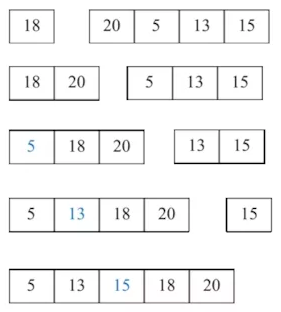
\includegraphics[scale=0.7]{ins_sort.png}}
		\caption{Сортировка вставками.}
		\label{fig:ins_s}
	\end{figure}
	
	\newpage
	
	\section{Сортировка выбором}
	Общая идея алгоритма состоит в следующем \cite{select}:
	
	\begin{itemize}
		\item в неотсортированном подмассиве ищется локальный максимум (минимум);
		\item найденный максимум (минимум) меняется местами с последним (первым) элементом в подмассиве;
		\item делать так, пока в массиве остались неотсортированные подмассивы.
	\end{itemize}
	
	\section{Вывод}
	В данном разделе была проанализирована предметная область и рассмотрены 3 алгоритма сортировки: пузырьком, вставками и выбором.
	
	Входными данными для программы являются:
	
	\begin{itemize}
		\item длина массива;
		\item массив действительных чисел.
	\end{itemize}
	
	Выходные данные: отсортированный по возрастанию массив.
	
	Ограничения, в рамках которых будет работать программа:
	
	\begin{itemize}
		\item элементами массива являются действительные числа;
		\item массив сортируется по возрастанию;
		\item корректность данных в пользовательском разделе не проверяется.
	\end{itemize}
	
	Функциональные требования к ПО:
	
	\begin{itemize}
		\item ПО должно содержать 2 раздела: пользовательский (ручной ввод) и экспериментальный (для замеров времени);
		\item ПО должно выводить отсортированный массив;
		\item ПО должно выводить потраченное время.
	\end{itemize}
	
	\clearpage
	
	\chapter{Конструкторская часть}
	
	В этом разделе на основе теоретических данных, полученных в аналитическом разделе, будут построены схемы исследуеммых алгоритмов. А также будут описаны: структуры данных, используемые в алгоритмах, способы тестирования и классы эквивалентности, память, используемая алгоритмом, и структура ПО.
	
	\section{Схемы алгоритмов}
	На рисунках \ref{fig:bubble} - \ref{fig:sel} представлены схемы рассматриваемых алгоритмов.
	
	\begin{figure}[h]
		\centering
		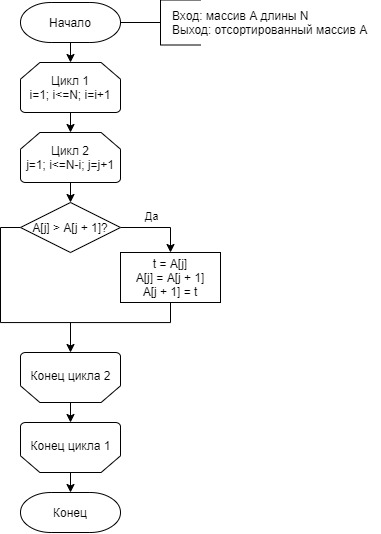
\includegraphics[width=0.5\linewidth]{bsort.jpg}
		\caption{Схема сортировки пузырьком}
		\label{fig:bubble}
	\end{figure}
	
	\newpage
	
	\begin{figure}[h]
		\centering
		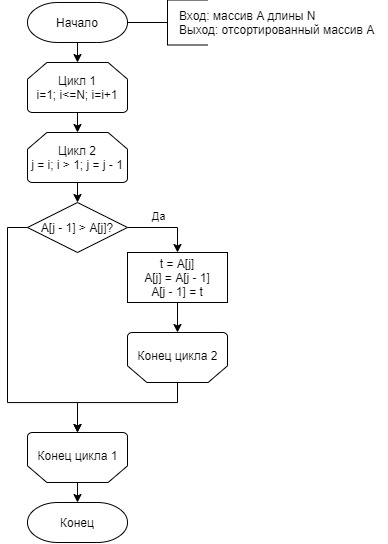
\includegraphics[scale=0.9]{isort.jpg}
		\caption{Схема сортировки вставками}
		\label{fig:ins}
	\end{figure}
	
	\newpage
	
	\begin{figure}[h]
		\centering
		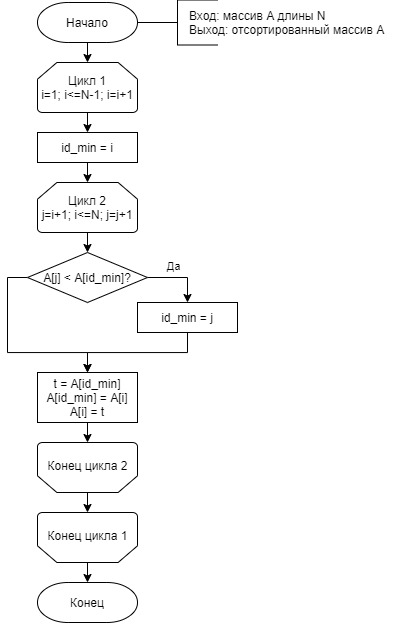
\includegraphics[scale=0.8]{ssort.jpg}
		\caption{Схема сортировки выбором}
		\label{fig:sel}
	\end{figure}
	
	\newpage
	
	\section{Модель вычислений}
	
	Для последующего вычисления трудоемкости введём модель вычислений:
	
	\begin{enumerate}
		\item Операции из списка (\ref{for:opers}) имеют трудоемкость 1.
		\begin{equation}
			\label{for:opers}
			+, -, /, \%, ==, !=, <, >, <=, >=, [], ++, {-}-
		\end{equation}
		\item Трудоемкость оператора выбора if условие then A else B рассчитывается, как (\ref{for:if}).
		\begin{equation}
			\label{for:if}
			f_{if} = f_{\text{условия}} +
			\begin{cases}
				f_A, & \text{если условие выполняется,}\\
				f_B, & \text{иначе.}
			\end{cases}
		\end{equation}
		\item Трудоемкость цикла рассчитывается, как (\ref{for:for}).
		\begin{equation}
			\label{for:for}
			f_{for} = f_{\text{инициализации}} + f_{\text{сравнения}} + N(f_{\text{тела}} + f_{\text{инкремента}} + f_{\text{сравнения}})
		\end{equation}
		\item Трудоемкость вызова функции равна 0.
	\end{enumerate}
	
	\section{Трудоёмкость алгоритмов}
	
	Пусть размер массивов во всех вычислениях обозначается как $N$.
	
	\subsection{Алгоритм сортировки пузырьком}
	
	Трудоёмкость алгоритма сортировки пузырьком состоит из:
	\begin{itemize}
		\item трудоёмкость сравнения и инкремента внешнего цикла $i \in [1..N)$ (\ref{for:bubble_outer}):
		\begin{equation}
			\label{for:bubble_outer}
			f_{i} = 2 + 2(N - 1)
		\end{equation}
		\item суммарная трудоёмкость внутренних циклов, количество итераций которых меняется в промежутке $[1..N-1]$ (\ref{for:bubble_inner}):
		\begin{equation}
			\label{for:bubble_inner}
			f_{j} = 3(N - 1) + \frac{N \cdot (N - 1)}{2} \cdot (3 + f_{if})
		\end{equation}
		\item трудоёмкость условия во внутреннем цикле (\ref{for:bubble_if}):
		\begin{equation}
			\label{for:bubble_if}
			f_{if} = 4 + \begin{cases}
				0, & \text{в лучшем случае}\\
				9, & \text{в худшем случае}\\
			\end{cases}
		\end{equation}
	\end{itemize}
	
	Трудоёмкость в \textbf{лучшем} случае (\ref{for:bubble_best}):
	\begin{equation}
		\label{for:bubble_best}
		f_{best} = \frac{7}{2} N^2 + \frac{3}{2} N - 3 \approx \frac{7}{2} N^2 = O(N^2)
	\end{equation}
	
	Трудоёмкость в \textbf{худшем} случае (\ref{for:bubble_worst}):
	\begin{equation}
		\label{for:bubble_worst}
		f_{worst} =  8N^2 - 8N - 3 \approx 8N^2 = O(N^2)
	\end{equation}
	
	\subsection{Алгоритм сортировки вставками}
	
	Трудоёмкость алгоритма сортировки пузырьком состоит из:
	\begin{itemize}
		\item трудоёмкость сравнения и инкремента внешнего цикла $i \in [1..N)$ (\ref{for:isort_outer}):
		\begin{equation}
			\label{for:isort_outer}
			f_{i} = 2 + 2(N - 1)
		\end{equation}
		\item суммарная трудоёмкость внутренних циклов, количество итераций которых меняется в промежутке $[1..N-1]$ (\ref{for:isort_inner}):
		
		\begin{equation}
			\label{for:isort_inner}
			f_{if} = 4 + \begin{cases}
				0, & \text{в лучшем случае}\\
				3(N - 1) + \frac{N \cdot (N - 1)}{2} \cdot (3 + f_{if}), & \text{в худшем случае}\\
			\end{cases}
		\end{equation}
		
		\item трудоёмкость условия во внутреннем цикле (\ref{for:isort_if}):
		\begin{equation}
			\label{for:isort_if}
			f_{if} = 4 + \begin{cases}
				0, & \text{в лучшем случае}\\
				9, & \text{в худшем случае}\\
			\end{cases}
		\end{equation}
	\end{itemize}
	
	Трудоёмкость в \textbf{лучшем} случае (\ref{for:isort_best}):
	\begin{equation}
		\label{for:isort_best}
		f_{best} = 13N - 10 \approx 13N = O(N)
	\end{equation}
	
	Трудоёмкость в \textbf{худшем} случае (\ref{for:isort_worst}):
	\begin{equation}
		\label{for:isort_worst}
		f_{worst} = 4.5N^2 + 10N - 13 \approx 4N^2 = O(N^{2})
	\end{equation}

	\section{Структуры данных}
	В данной работе из структур данных используются только одномерные массивы.
	
	\section{Тестирование и классы эквивалентности}
	Для проверки работоспособности ПО будет применяться функциональное тестирование.
	
	Классы эквивалентности:
	
	\begin{itemize}
		\item массив уже отсортирован по возрастанию;
		\item массив отсортирован в обратном порядке;
		\item массив никак не отсортирован;
		\item массив из одного элемента;
		\item пустой массив.
	\end{itemize}
	
	\section{Используемая память}
	Все используемые в данной работе массивы будут динамическими. В связи с этим, нужно будет контролировать проблемы с памятью, в частности при выделении памяти под массивы и её освобождении из-под них.
	
	Из всего вышесказанного следует, что количество памяти, необходимой алгоритмам, пропорционально длинам массивов.
	
	\section{Структура ПО}
	ПО будет состоять из набора функций:
	
	\begin{itemize}
		\item основная функция, работающая с меню;
		\item ввод исходных данных с клавиатуры;
		\item сортировка пузырьком;
		\item сортировка вставками;
		\item сортировка выбором;
		\item замеры времени.
	\end{itemize}
	
	\section{Вывод}
	На основе теоретических данных, полученные в аналитическом разделе были построены схемы иследуеммых  алгоритмов и оценены их трудоёмкости в лучшем и худшем случае. Также были описаны: структуры данных, используемые в алгоритмах, способы тестирования и классы эквивалентности, память, используемая алгоритмом, и структура ПО.
	
	\chapter{Технологическая часть}
	
	В этом разделе будут разработаны исходные коды трёх алгоритмов сортировки: пузырьком, вставками и выбором.
	
	\section{Средства реализации}
	Для реализации программы сортировки массивов был выбран язык программирования Python. Данный выбор обусловлен тем, что в этом языке присутсвует функция для измерения процессорного времени.
	
	\section{Реализация алгоритмов}
	
	В листингах \ref{bubble} - \ref{select} приведена реализация трёх алгоритмов сортировки.
	
	\begin{lstlisting}[label=bubble,caption=Функция сортировки пузырьком,language=Python]
		def bubble_sort(arr, n):
			res = [arr[x] for x in range(n)]
			for i in range(n):
				for j in range(n - i - 1):
					if res[j] > res[j + 1]:
						res[j], res[j + 1] = res[j + 1], res[j]
			return res
	\end{lstlisting}
	
	\begin{lstlisting}[label=insert,caption=Функция сортировки вставками,language=Python]
		def insert_sort(arr, n):
			res = [arr[x] for x in range(n)]
			for i in range(n):
				current = res[i]
				j = i
				while (res[j - 1] > current) and (j > 0):
					res[j] = res[j - 1]
					j -= 1
				res[j] = current
			return res
	\end{lstlisting}

	\newpage
	
	\begin{lstlisting}[label=select,caption=Функция сортировки выбором,language=Python]
		def select_sort(arr, n):
			res = [arr[x] for x in range(n)]
			for i in range(n - 1):
				id_min = i
				for j in range(i + 1, n):
					if res[j] < res[id_min]:
						id_min = j
				res[i], res[id_min] = res[id_min], res[i]
			return res
	\end{lstlisting}
	
	\section{Тестовые данные}
	
	В таблице~\ref{tbl:test} приведены тесты для функций, реализующих алгоритмы сортировки. Все тесты пройдены успешно.
	
	\begin{table}[h!]
		\begin{center}
			\caption{\label{tbl:test}Тестирование функций}
			\begin{tabular}{|c|c|c|}
				\hline
				Входной массив & Результат & Ожидаемый результат \\ 
				\hline
				$[1, 3, 5, 7, 9]$ & $[1, 3, 5, 7, 9]$  & $[1, 3, 5, 7, 9]$\\\hline
				$[9, 7, 5.34, 3, 1]$  & $[1, 3, 5.34, 7, 9]$ & $[1, 3, 5.34, 7, 9]$\\\hline
				$[-7, 5, 9, -3, -1]$  & $[-7, -3, -1, 5, 9]$  & $[-7, -3, -1, 5, 9]$\\\hline
				$[10.2]$  & $[10.2]$  & $[10.2]$\\\hline
				Пустой массив  & Пустой массив  & Пустой массив\\
				\hline
			\end{tabular}
		\end{center}
	\end{table}
	
	\section{Вывод}
	В данном разделе были разработаны исходные коды трёх алгоритмов сортировки: пузырьком, вставками и выбором.
	
	\chapter{Исследовательская часть}
	
	В этом разделе будет проведён эксперимент для определения эффективности по времени работы каждого из разработанных алгоритмов.
	
	\section{Пример работы}
	
	Демонстрация работы программы приведена на рисунке 4.1.
	
	\begin{figure}[h]
		\begin{center}
			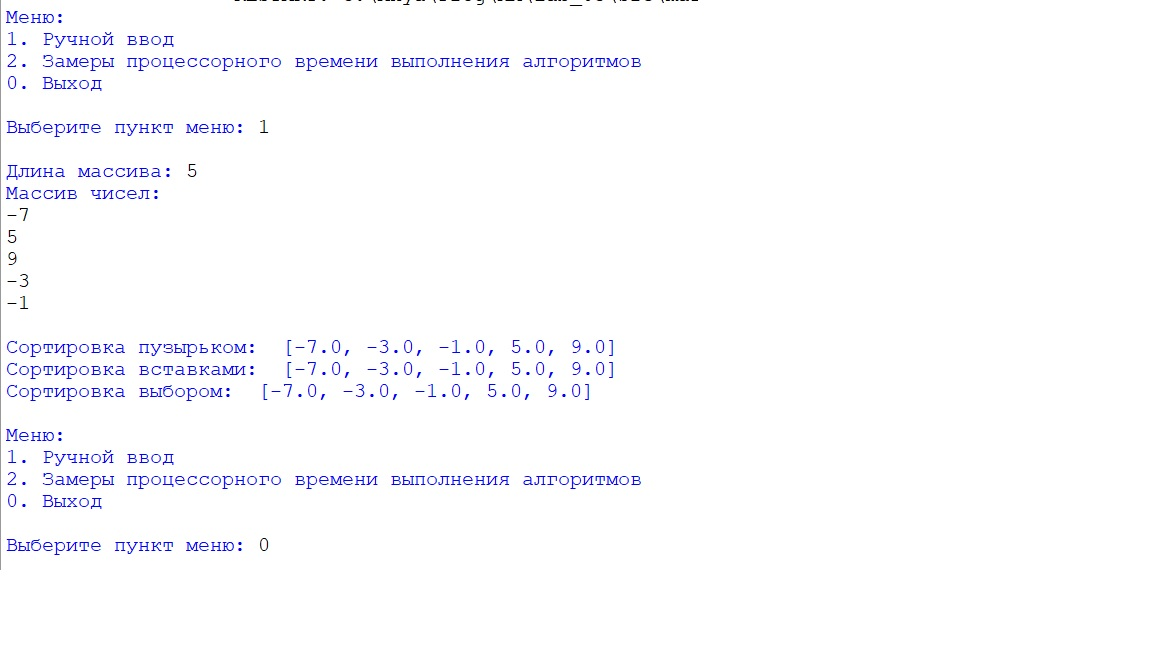
\includegraphics[scale=1]{example.jpg}
			\caption{Работа алгоритмов сортировки}
		\end{center}
	\end{figure}

	\section{Технические характеристики}
	
	Ниже приведеные технические характеристики устройства, на котором было проведенно тестирование ПО:
	
	\begin{itemize}
		
		\item Операционная система: Windows 10 64-bit Home \cite{home}.
		
		\item Оперативная память: 8 GB.
		
		\item Процессор: 11th Gen Intel(R) Core(TM) i3-1115G4 @ 3.00GHz
		\cite{i3}.
		
	\end{itemize}
	
	\section{Время выполнения алгоритмов}
	Время выполнения алгоритмов замерялось с помощью функции process\_time модуля time в Python  \cite{process}. Данная функция возвращает значение в долях секунды суммы системного и пользовательского процессорного времени текущего процесса. \newline
	
	В таблицах 4.1 - 4.3 представлены замеры времени работы для каждого из алгоритмов.
	
	\begin{table} [h!]
		\caption{Время выполнения отсортированных по возрастанию данных (лучший случай)}
		\begin{center}
			\begin{tabular}{|c c c c|}
				\hline
				Размер & Пузырёк & Вставки  & Выбор \\
				\hline
				100 & 0.000313 & 0 & 0.000313 \\ 
				\hline 
				300 & 0.002188 & 0 & 0.001719 \\ 
				\hline 
				500 & 0.006094 & 0 & 0.004844 \\ 
				\hline 
				700 & 0.012031 & 0 & 0.009844 \\ 
				\hline 
				900 & 0.020625 & 0 & 0.016250 \\ 
				\hline 
				1100 & 0.030937 & 0.000156 & 0.024375 \\ 
				\hline 
				1300 & 0.044531 & 0.000156 & 0.034063 \\ 
				\hline 
				1500 & 0.059062 & 0.000156 & 0.045937 \\ 
				\hline 
				1700 & 0.076406 & 0.000156 & 0.057656 \\ 
				\hline 
				1900 & 0.095781 & 0.000156 & 0.072500 \\ 
				\hline 
				2100 & 0.117969 & 0.000313 & 0.087656 \\ 
				\hline 
			\end{tabular}
		\end{center}
	\end{table}

	\begin{table} [h!]
		\caption{Время выполнения отсортированных по убыванию данных (худший случай)}
		\begin{center}
			\begin{tabular}{|c c c c|}
				\hline
				Размер & Пузырёк & Вставки  & Выбор \\
				\hline
				100 & 0.000625 & 0.000469 & 0.000313 \\ 
				\hline 
				300 & 0.005469 & 0.004219 & 0.001875 \\ 
				\hline 
				500 & 0.015625 & 0.012188 & 0.005313 \\ 
				\hline 
				700 & 0.031563 & 0.024688 & 0.010156 \\ 
				\hline 
				900 & 0.052969 & 0.041875 & 0.016875 \\ 
				\hline 
				1100 & 0.080469 & 0.063594 & 0.025469 \\ 
				\hline 
				1300 & 0.112500 & 0.089375 & 0.035469 \\ 
				\hline 
				1500 & 0.153125 & 0.120781 & 0.047969 \\ 
				\hline 
				1700 & 0.201719 & 0.156406 & 0.060937 \\ 
				\hline 
				1900 & 0.253125 & 0.197500 & 0.076563 \\ 
				\hline 
				2100 & 0.303594 & 0.240156 & 0.093125 \\ 
				\hline 
			\end{tabular}
		\end{center}
	\end{table}

	\begin{table} [h!]
		\caption{Время выполнения алгоритмов на случайных данных}
		\begin{center}
			\begin{tabular}{|c c c c|}
				\hline
				Размер & Пузырёк & Вставки  & Выбор \\
				\hline
				100 & 0.000469 & 0.000313 & 0.000313 \\ 
				\hline 
				300 & 0.004219 & 0.002344 & 0.002031 \\ 
				\hline 
				500 & 0.012344 & 0.006719 & 0.005625 \\ 
				\hline 
				700 & 0.023906 & 0.013594 & 0.010937 \\ 
				\hline 
				900 & 0.040469 & 0.022656 & 0.017969 \\ 
				\hline 
				1100 & 0.060937 & 0.033906 & 0.026719 \\ 
				\hline 
				1300 & 0.085000 & 0.047500 & 0.036719 \\ 
				\hline 
				1500 & 0.113906 & 0.063750 & 0.049063 \\ 
				\hline 
				1700 & 0.146875 & 0.081250 & 0.063125 \\ 
				\hline 
				1900 & 0.184375 & 0.102031 & 0.078437 \\ 
				\hline 
				2100 & 0.225469 & 0.124531 & 0.095469 \\ 
				\hline 
			\end{tabular}
		\end{center}
	\end{table}

	\newpage

	\begin{figure}[h!]
		\begin{center}
			\begin{tikzpicture}
				\begin{axis}[
					legend pos = north west,
					xlabel=длина строки,
					ylabel=секунды,
					minor tick num = 1,
					grid = both,
					major grid style = {lightgray},
					minor grid style = {lightgray!25},
					xtick distance = 100,
					width = 0.9\textwidth,
					height = 0.5\textwidth]
					
					\addplot[
					blue,
					semithick,
					mark = x,
					mark size = 3pt,
					thick,
					] file {bbest.txt};
					
					\addplot[
					red,
					semithick,
					mark = *,
					] file {ibest.txt};
					
					\addplot[
					green,
					semithick,
					mark = *,
					] file {sbest.txt};
					
					\legend{
						Пузырёк,
						Вставки,
						Выбор
					}
				\end{axis}
			\end{tikzpicture}
		\end{center}
		\caption{Сравнение алгоритмов сортировки пузырьком, вставками и выбором на лучшем случае}
	\end{figure}
	
	\begin{figure}[h!]
		\begin{center}
			\begin{tikzpicture}
				\begin{axis}[
					legend pos = north west,
					xlabel=длина строки,
					ylabel=секунды,
					minor tick num = 1,
					grid = both,
					major grid style = {lightgray},
					minor grid style = {lightgray!25},
					xtick distance = 100,
					width = 0.9\textwidth,
					height = 0.5\textwidth]
					
					\addplot[
					blue,
					semithick,
					mark = x,
					mark size = 3pt,
					thick,
					] file {bubble.txt};
					
					\addplot[
					red,
					semithick,
					mark = *,
					] file {insert.txt};
					
					\addplot[
					green,
					semithick,
					mark = *,
					] file {select.txt};
					
					\legend{
						Пузырёк,
						Вставки,
						Выбор
					}
				\end{axis}
			\end{tikzpicture}
		\end{center}
		\caption{Сравнение алгоритмов сортировки пузырьком, вставками и выбором на случайных данных}
	\end{figure}
	
	\newpage
	
	\section{Вывод}
	
	В лучшем случае (на отсортированном по возрастанию массиве) быстрее всего работает сортировка вставками, а медленнее всего - пузырьком (сортировка выбором эффективнее пузырька в среднем примерно на 16,3\%).
	
	На случайных данных быстрее всего работает сортировка выбором. Она эффективнее сортировки вставками в среднем примерно на 14\% и эффективнее сортировки пузырьком в среднем примерно на 50\%.
	
	
	\chapter*{Заключение}
	\addcontentsline{toc}{chapter}{Заключение}
	
	На основании анализа трудоемкости алгоритмов в выбранной модели вычислений, было показано, что алгоритм сортировки вставками имеет наименьшую сложность (линейную) в уже отсортированном массиве. В случае обратно отсортированного массива, сортировка вставками и пузырьком имееют квадратическую сложность. На основании замеров времени исполнения алгоритмов, был сделан вывод, что при прямом порядке элементов в массиве, сортировка пузьком работает медленее, чем выбором (примерно на 16,3\%). Так же был доказана выведенная трудоемкость алгоритма сортировки вставками - при  уже отсортированном массиве сортировка работает очень быстро, она является в таком случае наиболее эффективной. На случайных же данных быстрее всех работает алгоритм сортировки выбором.
	
	\addcontentsline{toc}{chapter}{Список литературы}
	
	\bibliographystyle{utf8gost705u}  % стилевой файл для оформления по ГОСТу
	
	\bibliography{biblio}          % имя библиографической базы (bib-файла)
	
\end{document}